\section{Rupture: An improved attack}\label{subsec:rupture}
Our first contribution is the development of a production-grade framework called
Rupture, which was developed as part of the work on extending the BREACH attack
against modern systems.

Rupture provides extended functionality regarding the network aspects of the
attack. It offers the ability to inject malicious code in any computer on the
network, perform traffic inspection and analyze captured data.

\subsection{Attack design}\label{subsec:rupture_attack_design}

Rupture enables the automated computation of the reflection strings in each
round of the attack. For this computation, the adversary should firstly know a
prefix of the secret, which is needed to build the initial reflections and
bootstrap the attack.

Each reflection consists of the known prefix concatenated with a character in
the candidate alphabet. The candidate alphabet initially is equal to the
alphabet of the secret and, as the attack progresses, it may be reduced to a
smaller set of symbols. This construction method ensures that a reflection $r_i$
in the reflection vector $\bar{r} = <r_1, r_2, ...>$ will match the secret.

The adversary issues consecutive requests, each containing a different
reflection. The goal is to recognize the one that matches secret, which is
achieved by exploiting the way most compression functions like DEFLATE behave.

In the case when $r$ matches the secret $s$, the compression will be better than
a case of no-match. Therefore, the network response packets for the matching
reflection will be smaller than the packets of the incorrect reflections.

We define a \textit{sample} as the encrypted data pertaining to one response for
a single reflection. The set of samples collected for a particular reflection is a
\textit{sampleset}. The collected samplesets for all candidates in the alphabet
form a \textit{batch}.

The attack is conducted in \textit{rounds}. In each round, a decision is made
about the state of the attack, so either the next byte of the secret becomes
known or the candidate alphabet is drilled down to a smaller set. Rupture
amplifies the results by using multiple samples in each
sampleset in order to achieve better probability of success. Therefore during the
analysis Rupture collects a batch's samplesets, compares the mean length of the
responses for all candidates, and chooses the candidate with the smaller mean
response length as the correct one.

This decision is made with some \textit{confidence} which is expressed in bytes.
If the confidence is insufficient, an additional batch is collected and the
analysis is redone using the aggregated lengths from all collected batches.

Once enough batches have been collected for a decision to be made with good
confidence, the round of the attack is complete.  Each stage of the attack
consists of one or more rounds and is concluded by decrypting a single byte of the
secret.

\subsection{Architecture}\label{app:rupture}
Rupture is a service-based architecture framework which contains multiple
independent components. The components are able to run on
different networks, although the attack can be easily launched by running all
modules on a single system.

The framework assumes a \textit{target} service to be attacked. This target is a
web service which uses TLS and provides HTTPS endpoints as described in section
\ref{subsec:example}. However, we have designed Rupture to be a good playground
for experimentation with new attacks, so this assumption can be relaxed and
attacks against other similar protocols are possible. Examples of other
encrypted protocols that can be explored in future work include SMTP and XMPP.

The framework also assumes the \textit{victim}, a user who is associated with
the particular target and whose data will be decrypted. Both the target and the
victim are modeled with various attributes and are easily configurable.

There are two underlying assumptions in our attack: the injection and the
sniffing. These are often, but not necessarily, achieved through the same means.
The injection assumption states that the adversary is able to inject code, the
\textit{client}, to the victim's machine for execution. This code is able to
issue adaptive requests to the target service. The sniffing assumption states
that the adversary is able to observe encrypted network traffic between the
victim and the target. Although a passive network access for the adversary
covers the sniffing assumption, in the cases where injection is needed the
adversary should have active network access.

Rupture's architecture is depicted in figure \ref{fig:rupture_architecture} and
the various components that implement the above are described in detail in the
following paragraphs.

   \begin{figure}[thpb]
      \centering
          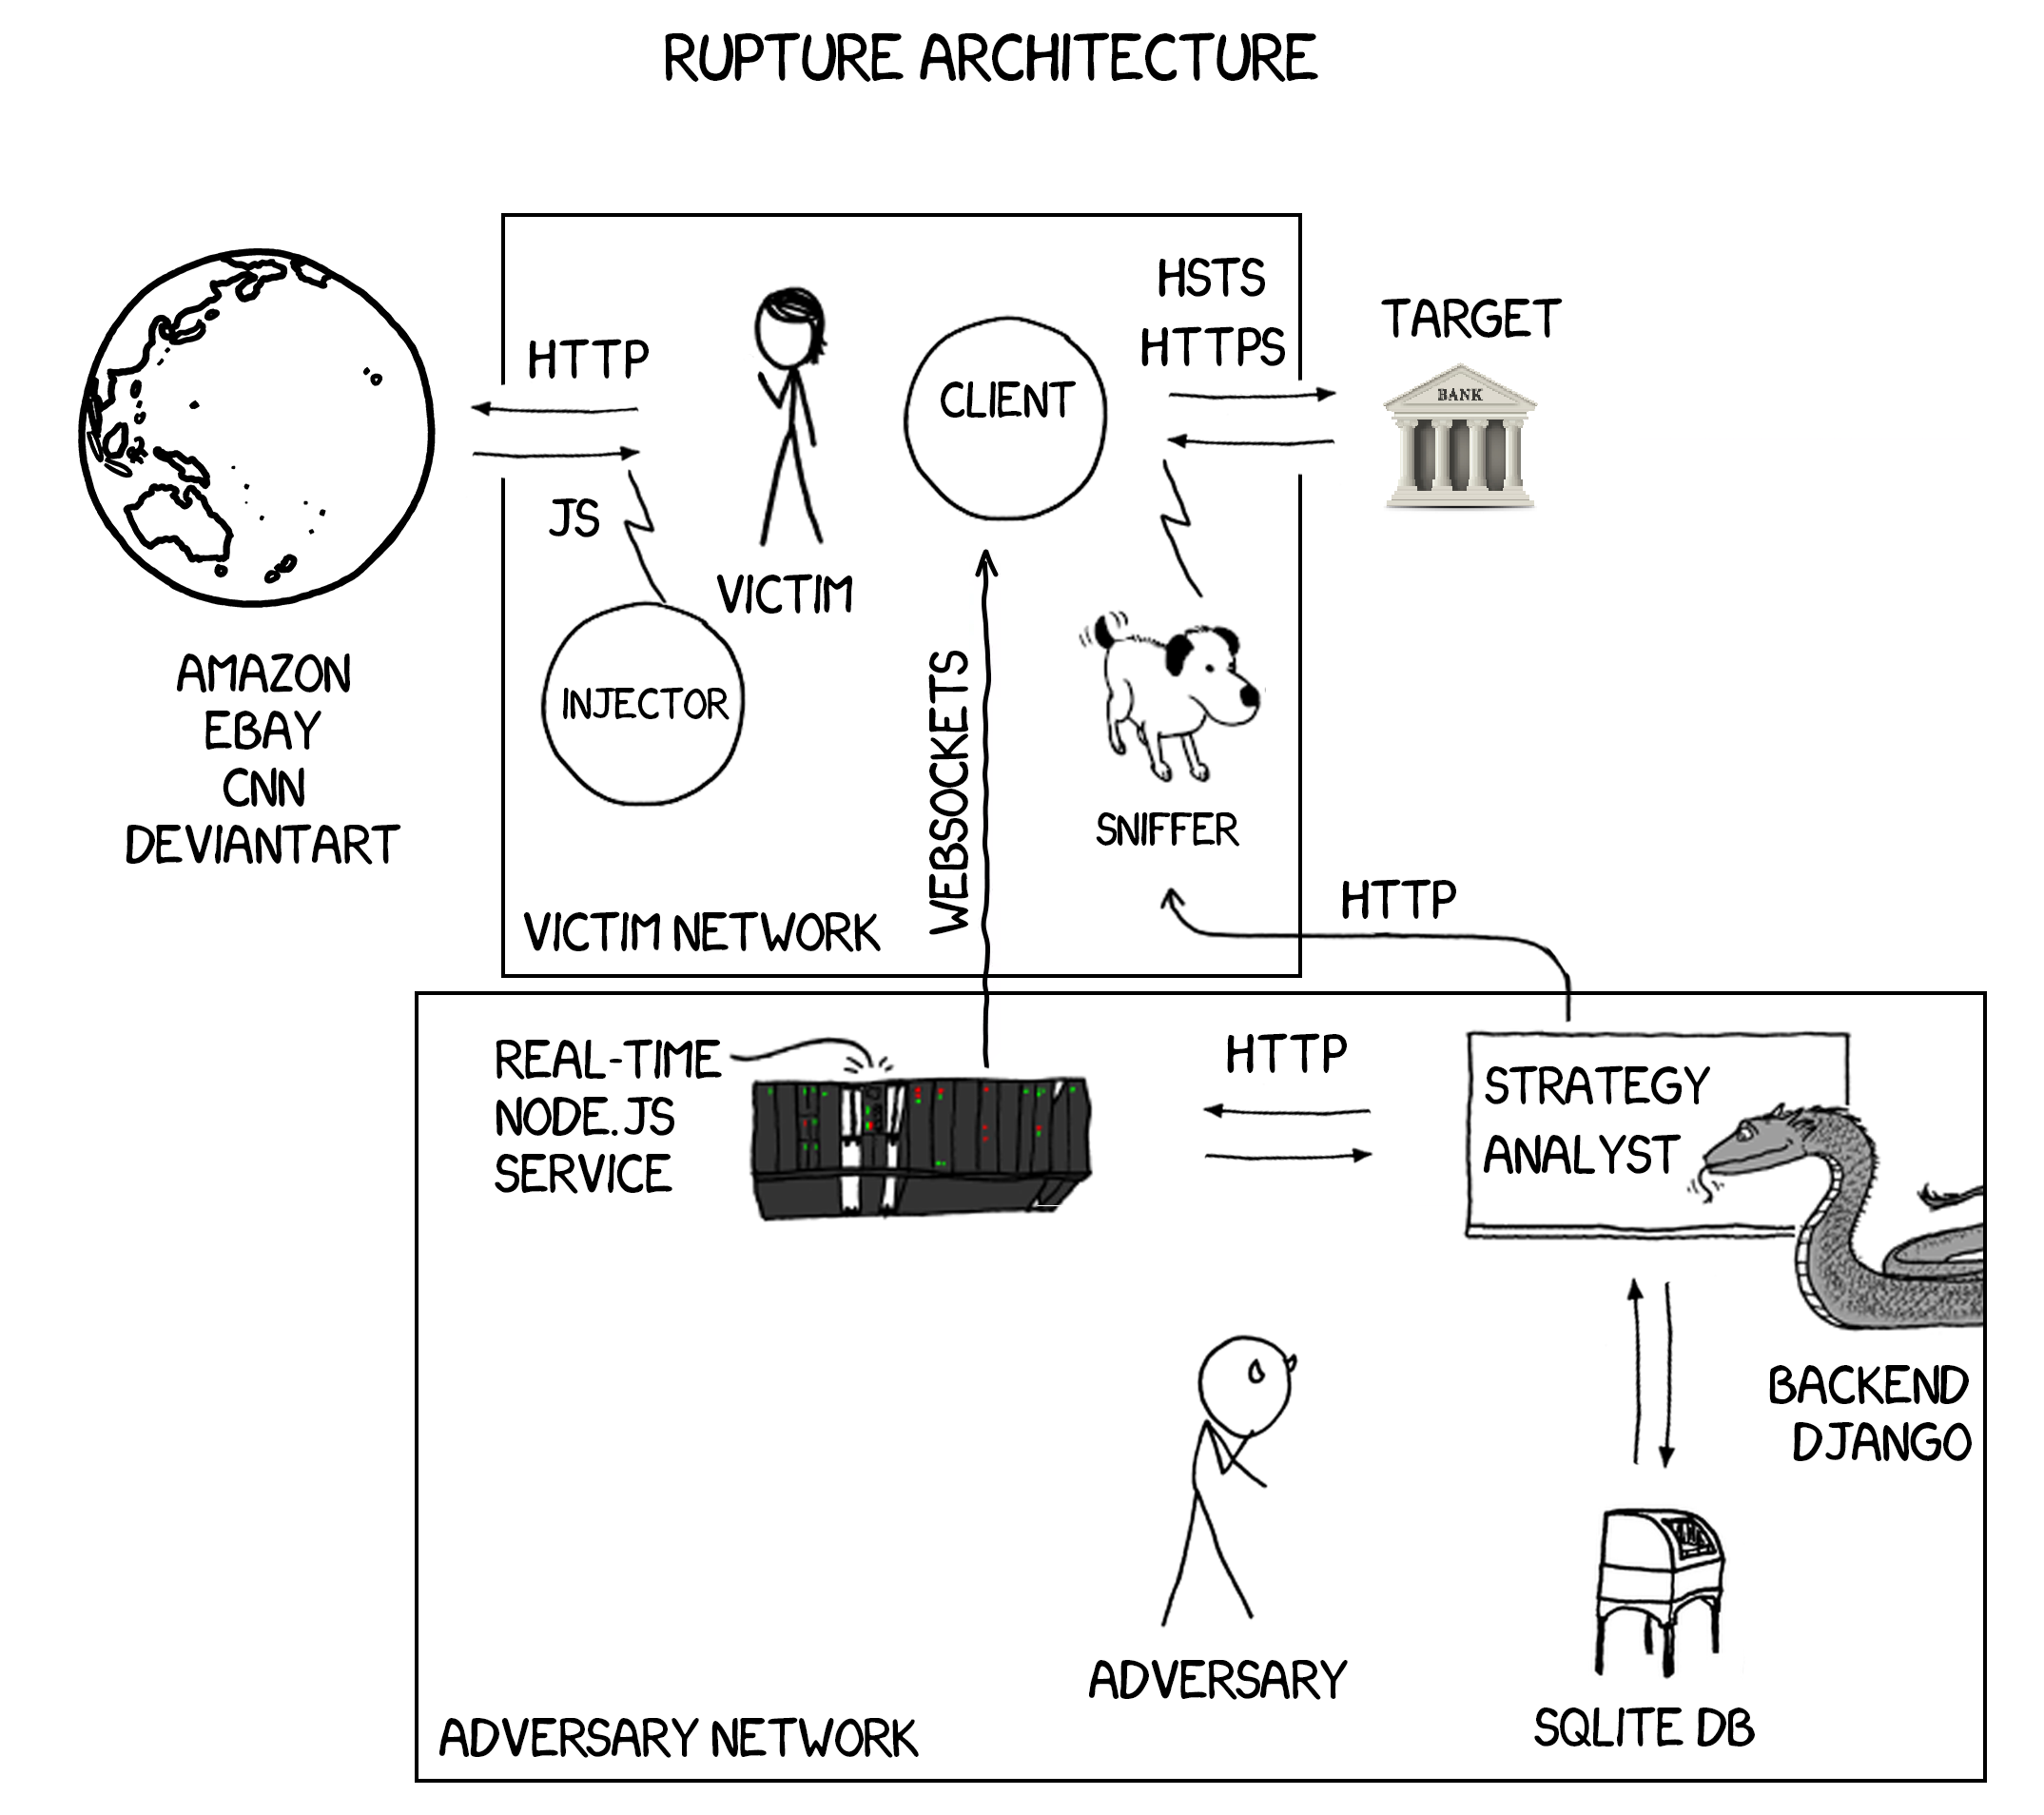
\includegraphics[width=0.48\textwidth]{figures/architecture.png}
      \caption{Rupture Architecture}
        \label{fig:rupture_architecture}
   \end{figure}

\subsubsection{Client}

The client component is a Javascript code that issues requests towards a chosen
endpoint. It needs to be executed from the browser of the victim, so that the
victim's authentication cookies are included in the request and the secrets are
included in the response. The client contains minimal logic by design. It
connects to the realtime service through a \textit{command-and-control} channel,
registers itself, and then waits for work instructions, which come in the form
of URLs for the requests it needs to make.

\subsubsection{Injector}

The injector component is responsible for injecting the client to the victim's
browser. The injection is performed by ARP spoofing (or NDP poisoning in the
case of IPv6) the local network and forwarding all traffic in a
Man-in-the-Middle manner. As the victim is browsing the Internet, multiple
clients will be injected in insecure pages and will run under various web contexts.
The fact that all HTTP responses are infected increases robustness,
as multiple injectors can be deployed to different networks, all controlled by the
same central command-and-control channel. The injector module is built using
Bettercap as the underlying tool for the network injection.

\subsubsection{Realtime}

The realtime is a service that acts as an intermediary between the clients and
the backend. When a client is injected in a page, it registers to the realtime and
maintains an open connection. Consequently the realtime holds command-and-control
connections with various clients which may live on different networks,
orchestrates them, and enforces the activation state for each one. It
activates one client per victim to receive work instructions and keeps the rest of
the victim's clients dormant. If the active client dies, for example by closing
its browser tab, one of the dormant clients is activated to continue the
attack. It also connects to the backend service using HTTP API calls to get
the work instructions for the active clients. The realtime is built in
Node.js \cite{tilkov2010node} and uses the socket.io framework
\cite{rai2013socket} for the command-and-control connections.

\subsubsection{Sniffer}

The sniffer component is responsible for collecting data from the victim's
network. When instructed, the sniffer collects the encrypted request and
response network packets for a given victim and a target. It also exposes a HTTP
API which is utilized by the backend for controlling when the sniffing starts and
stops, and to retrieve the sniffed data. It is built in Python, using Scapy
\cite{biondi2010scapy} for the network functionality.

\subsubsection{Backend}

The backend component is the center of operations for all attacks. It is
configured with the target and victim information, initializes the attacks and
designs the samplesets that should be collected.  When work needs to be done,
it forwards the instructions to the realtime in order to reach the clients. Meanwhile, it
orders the sniffer to listen for network traffic between the victim and the
target. When the client reports (via the realtime) that the work is completed, the
backend collects the traffic from the sniffer, analyzes the captured network
data and calculates the attack confidence for the round.
Therefore the backend is responsible for strategic decision taking and
adaptively advancing the attack. Based on statistical analysis of the network
samples, it decides if the collected samplesets are valid and if the confidence
is adequate for a round to be completed. It also stores persistent data about
the ongoing attack in a database for future analysis. It is built in Python,
using the Django framework for the RESTful API service.
